% PRL look and style (easy on the eyes)
\documentclass[aps,pre,twocolumn,nofootinbib,superscriptaddress,linenumbers]{revtex4-1}
% Two-column style (for submission/review/editing)
%\documentclass[aps,prl,preprint,nofootinbib,superscriptaddress,linenumbers]{revtex4-1}

%\usepackage{palatino}

% Change to a sans serif font.
\usepackage{sourcesanspro}
\renewcommand*\familydefault{\sfdefault} %% Only if the base font of the document is to be sans serif
\usepackage[T1]{fontenc}
%\usepackage[font=sf,justification=justified]{caption}
\usepackage[font=sf]{floatrow}

% Rework captions to use sans serif font.
\makeatletter
\renewcommand\@make@capt@title[2]{%
 \@ifx@empty\float@link{\@firstofone}{\expandafter\href\expandafter{\float@link}}%
  {\textbf{#1}}\sf\@caption@fignum@sep#2\quad
}%
\makeatother

\usepackage{listings} % For code examples
\usepackage[usenames,dvipsnames,svgnames,table]{xcolor}

\usepackage{amsmath}
\usepackage{amssymb}
\pdfoutput=1
\usepackage[pdftex]{graphicx}
%\usepackage[mathbf,mathcal]{euler}
%\usepackage{citesort}
\usepackage{dcolumn}
\usepackage{boxedminipage}
\usepackage{verbatim}
\usepackage[colorlinks=true,citecolor=blue,linkcolor=blue]{hyperref}


% The figures are in a figures/ subdirectory.
% \graphicspath{{figures/}}


% \newcommand{\pyitc}{\url{http://www.simtk.org/home/bayesian-itc}} % URL of pyITC project homepage

%% DOCUMENT %%%%%%%%%%%%%%%%%%%%%%%%%%%%%%%%%%%%%%%%%%%%%%%%%%%%%%%%%%%%%%%%%%%%
\begin{document}

%% TITLE %%%%%%%%%%%%%%%%%%%%%%%%%%%%%%%%%%%%%%%%%%%%%%%%%%%%%%%%%%%%%%%%%%%%
\title{Ensembler: Enabling high-throughput molecular simulations at the superfamily scale}

\author{Daniel L. Parton}
  \affiliation{Computational Biology Center, Memorial Sloan Kettering Cancer Center, New York, NY 10065}
  %\email{daniel.parton@choderalab.org}
\author{Patrick B. Grinaway}
  \affiliation{Computational Biology Center, Memorial Sloan Kettering Cancer Center, New York, NY 10065}
  %\email{patrick.grinaway@choderalab.org}
\author{John D. Chodera}
 \thanks{Corresponding author}
 \email{john.chodera@choderalab.org}
  \affiliation{Computational Biology Center, Memorial Sloan Kettering Cancer Center, New York, NY 10065}

\date{\today}

%%%%%%%%%%%%%%%%%%%%%%%%%%%%%%%%%%%%%%%%%%%%%%%%%%%%%%%%%%%%%%%%%%%%%%%%%%%%%%%%%%%%%%%%%%%%%%%%%%%%%%
% ABSTRACT/pacs
%%%%%%%%%%%%%%%%%%%%%%%%%%%%%%%%%%%%%%%%%%%%%%%%%%%%%%%%%%%%%%%%%%%%%%%%%%%%%%%%%%%%%%%%%%%%%%%%%%%%%%
\begin{abstract}

The rapidly expanding body of available genomic and protein structural data provides a rich resource for understanding protein dynamics with biomolecular simulation. 
However, simulations on an \emph{omics} scale are not yet widely performed, partly because software infrastructure to enable this has not kept pace. 
For example, it should now be possible to study protein dynamics across entire (super)families, exploiting the entire variety of available structural biology data and conformational similarities across homologous proteins.
Here, we present a new tool for enabling high-throughput simulation in the genomics era.
Ensembler takes any set of sequences---from a single sequence to an entire superfamily of interest---and shepherds them through various stages of modeling and refinement to produce simulation-ready structures.
This includes comparative modeling to all relevant PDB structures (which may span multiple conformational states of interest), reconstruction of missing loops, addition of missing atoms, culling of nearly identical structures, assignment of appropriate protonation states, solvation in explicit solvent, and refinement with molecular simulation to ensure stable simulation. 
The output of this pipeline is an ensemble of structures ready for subsequent parallel or distributed molecular simulations using clusters, supercomputers, or distributed computing projects like Folding@home.
Ensembler automates much of the time-consuming process of preparing protein models suitable for simulation, while allowing scalability up to entire superfamilies.  
A particular advantage of this approach can be found in the construction of kinetic models of conformational dynamics---such as Markov state models---which benefit from a diverse array of initial configurations that span the accessible conformational states to aid sampling.
We demonstrate the power of this approach by constructing models for all catalytic domains in the human tyrosine kinase family, using all available kinase catalytic domain structures from any organism as structural templates.

Ensembler is free of charge, and is made available under the terms of the GNU General Public License (GPL) v2. 
It should run on all major operating systems, and has been tested on Linux and OS X.
The latest release can be installed via the {\tt conda} package manager, and the latest source can be downloaded from \url{https://github.com/choderalab/ensembler}.

\emph{Keywords: molecular dynamics simulation; comparative modeling}

% TODO expand to all human protein kinases?

\end{abstract}

\maketitle

%%%%%%%%%%%%%%%%%%%%%%%%%%%%%%%%%%%%%%%%%%%%%%%%%%%%%%%%%%%%%%%%%%%%%%%%%%%%%%%%%%%%%%%%%%%%%%%%%%%%%%
% INTRODUCTION
%%%%%%%%%%%%%%%%%%%%%%%%%%%%%%%%%%%%%%%%%%%%%%%%%%%%%%%%%%%%%%%%%%%%%%%%%%%%%%%%%%%%%%%%%%%%%%%%%%%%%%
\section{Introduction}
\label{section:introduction}

Proteins play a diverse variety of roles in biology, and the understanding of their function---and how mutations can cause dysfunction and disease---is the preoccupation of much of modern biology. 
The diminishing cost of nucleic acid sequencing technologies has produced an enormous wealth of sequence data, yielding a large collection of protein-coding open reading frames that provide basic information about these proteins (at the level of primary amino acid sequences) for numerous organisms [CITE]. 
Complementing this, large-scale structural biology efforts such as the Protein Structure Initiative (PSI) and Structural Genomics Consortium (SGC) have yielded a great number of protein structures, allowing comparative modeling to provide insight into the static structures many of these proteins adopt [CITE review of structural biology efforts or current comparative modeling?].
% TODO Maybe it is not necessary to mention comparative modeling here? If so, this could be changed to:
% Complementing this, large-scale structural biology efforts such as the Protein Structure Initiative (PSI) and Structural Genomics Consortium (SGC) have provided insight into the static structures which these proteins can adopt [CITE review of structural biology efforts?].

Static structures, however, provide only a snapshot of the rich dynamical behavior of proteins.
Many functional properties---such as the ability to bind small molecules or interact with signaling partners---require conformational changes.

Molecular dynamics simulations have proven to be a useful tool for revealing the dynamics of individual proteins, with a number of software packages and forcefields available for biomolecular simulation.
Advances in computing architectures---especially the availability of GPUs, which provide a hundredfold increase in computational power per unit cost for a variety of applications---and the proliferation of scalable computing technologies (such as those that drive the Folding@home distributed computing resource [CITE]) now provide new hardware platforms on which to study the dynamics of these proteins.
In parallel, techniques for aggregating molecular dynamics simulation data to survey the kinetic landscape of biomolecules, such as Markov state modeling approaches [CITE MSM reviews], are now reaching maturity.

Despite this, a critical gap remains in the ability to bridge genome-scale sequence information and molecular simulations to enable the study of entire families or superfamilies of proteins in a single organism or across organisms. 
Molecular simulations must largely be set up by hand, with little in the way of automation available to provide practitioners a way of studying many members of a family where only a subset may have structural data.

Complicating matters further, in protein families known to be able to adopt multiple conformations---such as kinases---structural data may only exist for one or two conformations for any individual member of the family for which there is structural data.
This poses a challenge for biomolecular simulation methods such as Markov state models, which can provide detailed insight, but require global coverage of the conformational landscape to realize their full potential.

Here, we present the first steps toward a resolution of this problem: a fully automated open source framework for building simulation-ready protein models scalable to the superfamily scale.
We demonstrate the utility of this tool by constructing models for the entire set of human tyrosine kinase catalytic domains, and demonstrate that the resulting models provide good coverage of the known functional regions of structure space.
This tool forms the foundation for a new era of superfamily-scale molecular simulations for the Folding@home project.

%%%%%%%%%%%%%%%%%%%%%%%%%%%%%%%%%%%%%%%%%%%%%%%%%%%%%%%%%%%%%%%%%%%%%%%%%%%%%%%%%%%%%%%%%%%%%%%%%%%%%
% DESIGN AND IMPLEMENTATION
%%%%%%%%%%%%%%%%%%%%%%%%%%%%%%%%%%%%%%%%%%%%%%%%%%%%%%%%%%%%%%%%%%%%%%%%%%%%%%%%%%%%%%%%%%%%%%%%%%%%%
\section{Design and Implementation}

% Python
% Can be used via command-line tool Ensembler, or via the Python API

Ensembler is written in Python, and can be used via a command-line tool ({\tt ensembler}), or via the flexible Python API.

% Pipeline architecture, with a series of stages which must be performed in order.

The Ensembler modeling pipeline entails a series of stages which are performed in a defined order. 
A visual overview of the pipeline is shown in Fig.~\ref{figpipeline}, and a detailed description follows.

\begin{figure*}[h]
  \centering
    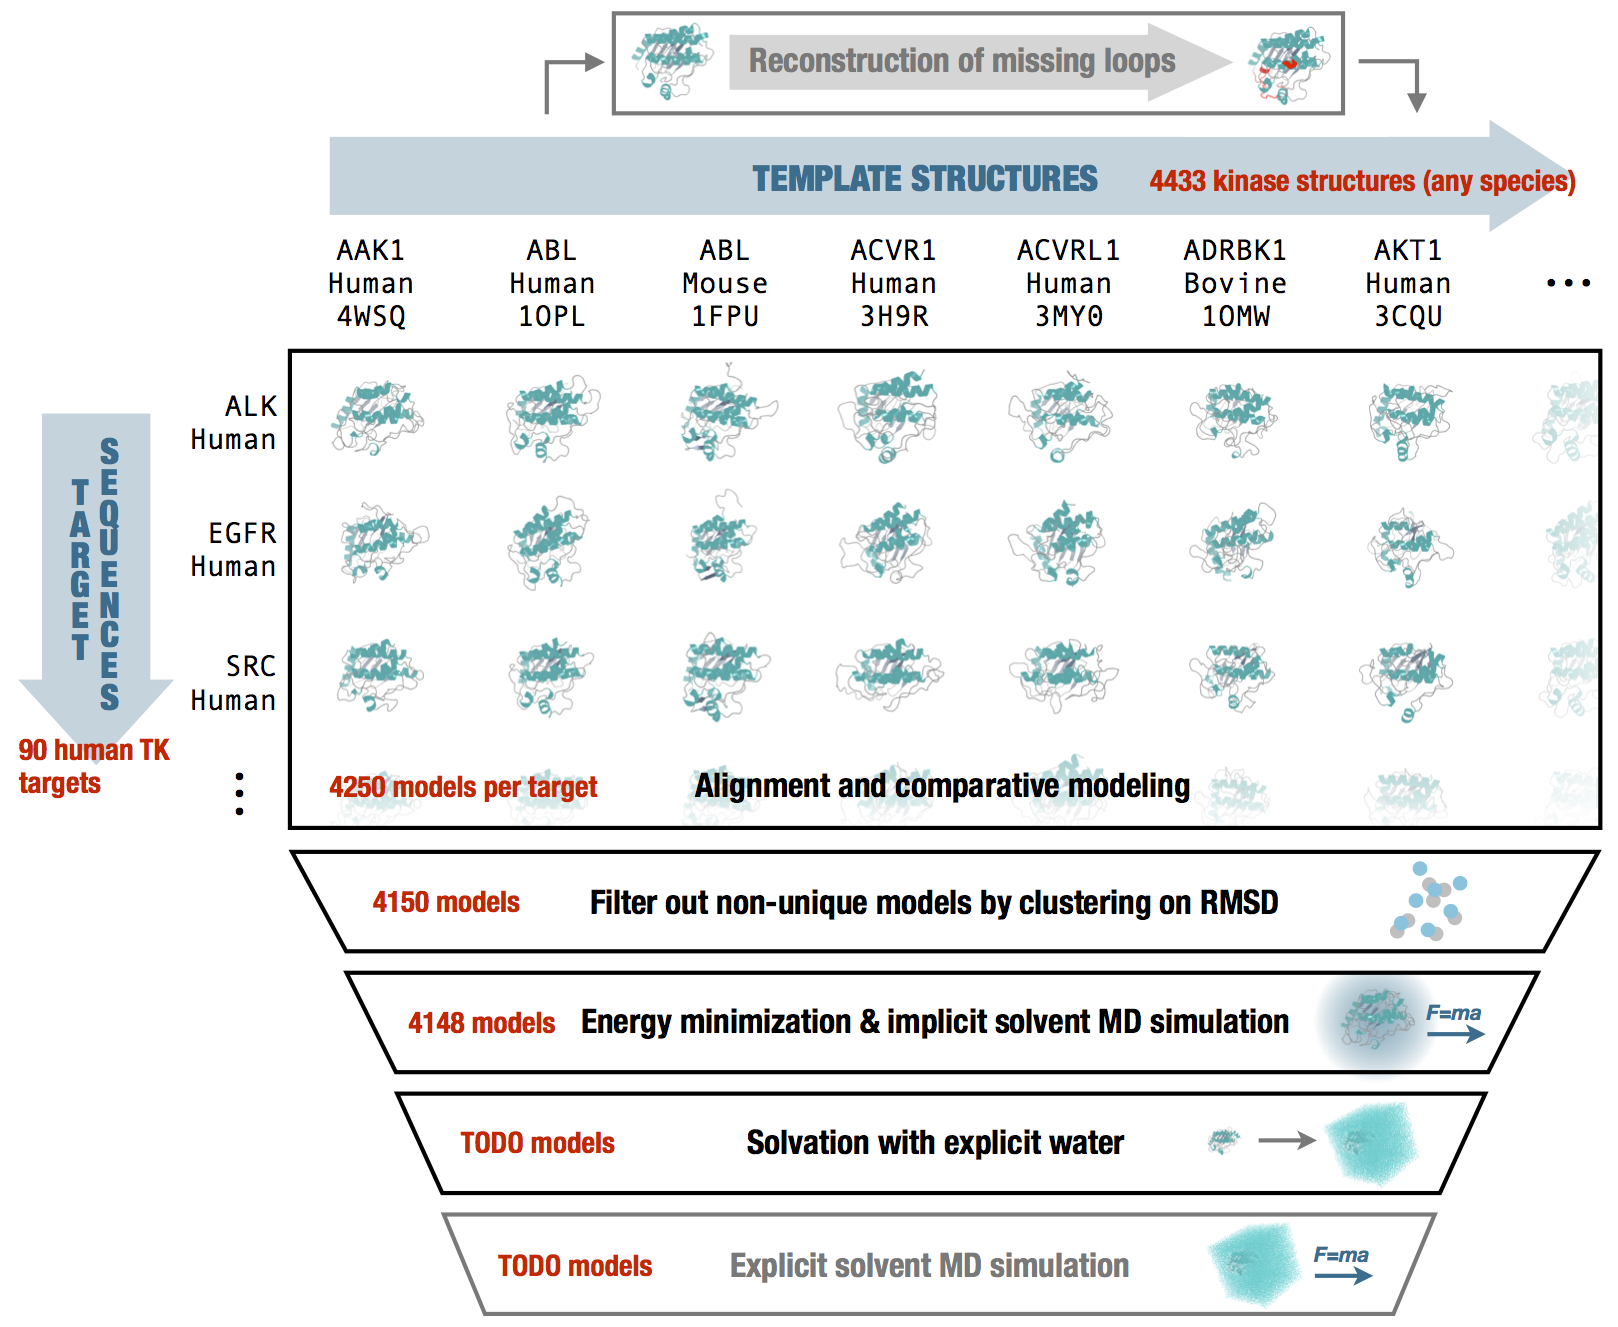
\includegraphics[width=0.8\textwidth]{pipeline}
  \caption{Ensembler pipeline}
  \label{figpipeline}
\end{figure*}

\subsubsection{Target selection}

The output from this stage is simply a FASTA-formatted sequence file containing the selected target sequences and identifiers. 
The {\tt ensembler} command-line tool provides methods for selecting targets from either UniProt (a freely accessible resource for protein sequence and functional data---\href{http://www.uniprot.org/}{uniprot.org}) or TargetExplorer (a database framework for aggregating various types of biological data; work to be published). 
This allows the user to easily select a single protein, many proteins, or an entire superfamily. Alternatively, the targets file can be generated using any other software, and stored at the appropriate filepath.

The method for selecting targets from UniProt is described here. 
A query string is required as input, using the same syntax as the search function on the UniProt website. 
For example, {\tt'domain:"Protein kinase" AND taxonomy:9606 AND reviewed:yes'} would select all human protein kinases which have been reviewed by a human curator. 
Ensembler is designed to work with protein \emph{domains}, rather than full-length proteins, and the desired protein domain(s) can be selected using a regular expression. 
For example, the string {\tt'\^{}Protein kinase(?!; truncated)(?!; inactive)'} would match domains annotated as "Protein kinase", "Protein kinase; 1" or "Protein kinase; 2", but would exclude the domains "Protein kinase; truncated" and "Protein kinase; inactive". 
The program then extracts sequences and identifiers from the UniProt data, and saves these to a FASTA-format text file.

% The selected targets are
% given identifiers of the form {\tt [UniProt mnemonic]\_D[domain index]}, which
% consists of the UniProt name for the target protein and a 0-based index for the
% domain (since a single target protein may contain multiple domains of
% interest). Example: {\tt EGFR\_HUMAN\_D0}.

\subsubsection{Template selection}

As for target selection, the {\tt ensembler} tool provides methods for selecting templates from various resources---UniProt, the Protein Data Bank (PDB; \href{http://www.pdb.org}{pdb.org}) or a TargetExplorer database.
From the user perspective, selection from UniProt proceeds in a similar fashion as described above.
The returned data for each UniProt entry includes an up-to-date list of PDB structures and their residue spans.
PDB files are downloaded from the PDB for structures which include the desired domain.
Data from the SIFTS service (\href{http://www.ebi.ac.uk/pdbe/docs/sifts/}{www.ebi.ac.uk/pdbe/docs/sifts}) (CITE: Velankar Nucleic Acids Res 2013), which provides residue-level mappings between PDB and UniProt entries, is then used to filter out PDB chains with $<$ 70\% resolved residues within the domain span.
Template sequences and structures are then extracted and written as FASTA-format sequence and PDB-format coordinate files respectively.

Selection from the PDB simply requires specifying a list of PDB IDs.
These are matched to UniProt entries via the SIFTS service, and the same procedure is then followed to extract template sequences and structures.

Unresolved template loops can optionally be remodeled with a kinematic closure algorithm, which is provided via the loopmodel tool of the Rosetta software suite (CITE: Rosetta and/or loopmodel).
This tends to provide higher-quality models following the subsequent modeling process.

\subsubsection{Modeling}

In this stage, models are generated for each target-template pair, using the Modeller automodel function (CITE: Modeller), which implements comparative structure modeling by satisfaction of spatial restraints (CITE: Sali Blundell J Mol Biol 1993; Fiser Sali Prot Sci 9 2000).
Modeller requires the user to first provide a target-template sequence alignment.
This is implemented in Ensembler using the BioPython {\tt pairwise2} module (CITE: BioPython)---which uses a dynamic programming algorithm---with the PAM 250 scoring matrix of Gonnet \textit{et al} (CITE: Gaston Gonnet Science 1992).

Non-unique models are then filtered out using structural similarity-based clustering.
The mdtraj (CITE: mdtraj) Python library is used to calculate RMSD with a fast quaternion characteristic polynomial (QCP) implementation, and the leader algorithm is then used to populate clusters.
A minimum distance cutoff (default: 0.6 \AA) is used to retain only a single model per cluster.

\subsubsection{Refinement}

Models are then refined with a steepest descent energy minimization and a short molecular dynamics (MD) simulation with implicit solvent.
This is implemented using the OpenMM molecular simulation toolkit (link and CITE: OpenMM), chosen for its flexible Python API, and high performance GPU-acclerated simulation code.
The Amber99SB-ILDN force field is used (CITE: amber99sbildn refs) with a modified generalized Born solvent model (GBSA-OBC) (CITE: GBSA-OBC).
The simulation is run for a default of 100 ps.
This refinement process helps to prepare models for subsequent production simulation, and also helps to filter out poor quality models.

Ensembler also provides optional routines for solvating models with explicit solvent and performing a second MD refinement.
The solvation step solvates each model for a given target with the same number of waters, as this is (currently) a requirement for building MSMs from multiple independent MD trajectories.
The target number of waters is selected by first solvating each model with a specified padding distance (default: 10 \AA), then taking a percentile value from the distribution (default: 68th percentile).
Models are resolvated with the target number of waters by first solvating with zero padding, then incrementally increasing the box size and resolvating until the target is exceeded, then finally deleting sufficient waters to match the target value.
The explicit solvent MD simulation is also implemented using OpenMM, with the Amber99SB-ILDN force field and TIP3P water.

\subsubsection{Packaging}

Finally, Ensembler provides a packaging module, which can be used to compress models in preparation for data transfer, or to prepare models with the appropriate directory and file structure for subsequent production simulations on the distributed computing platform Folding@Home (CITE: F@H).

\subsubsection{Other features}

% quickmodel function performs the entire pipeline in one go, for a single target and a small number of templates.
The command-line tool also provides a {\tt quickmodel} function, which performs the entire Ensembler pipeline for a single target with a small number of templates.
For larger numbers of models (such as entire protein families), the main pipeline functions should be used.
The modeling and refinement functions use MPI to trivially parallelize computation across each model (or across each template, in the case of the loop reconstruction code).

Each pipeline function also outputs a metadata file, which helps to link data to the software version used to generate it (both Ensembler and its dependencies), and also provides timing and performance information, and other data such as hostname.

% ? The API is highly flexible, allowing control over many important parameters. Appropriate choices have been set as default values.



% TODO where do these go?
% Distribution: conda package or github source
% Software is open source and designed to be extensible as far as possible. For example, it would be very simple to implement further options for providing target and template structures, or for packaging models.


\label{section:design}

%%%%%%%%%%%%%%%%%%%%%%%%%%%%%%%%%%%%%%%%%%%%%%%%%%%%%%%%%%%%%%%%%%%%%%%%%%%%%%%%%%%%%%%%%%%%%%%%%%%%%
% RESULTS
%%%%%%%%%%%%%%%%%%%%%%%%%%%%%%%%%%%%%%%%%%%%%%%%%%%%%%%%%%%%%%%%%%%%%%%%%%%%%%%%%%%%%%%%%%%%%%%%%%%%%
\section{Results}
\label{section:results}

%%%%%%%%%%%%%%%%%%%%%%%%%%%%%%%%%%%%%%%%%%%%%%%%%%%%%%%%%%%%%%%%%%%%%%%%%%%%%%%%%%%%%%%%%%%%%%%%%%%%%
% DISCUSSION
%%%%%%%%%%%%%%%%%%%%%%%%%%%%%%%%%%%%%%%%%%%%%%%%%%%%%%%%%%%%%%%%%%%%%%%%%%%%%%%%%%%%%%%%%%%%%%%%%%%%%
\section{Availability and Future Directions}
\label{section:availability}

%%%%%%%%%%%%%%%%%%%%%%%%%%%%%%%%%%%%%%%%%%%%%%%%%%%%%%%%%%%%%%%%%%%%%%%%%%%%%%%%%%%%%%%%%%%%%%%%%%%%%
% ACKNOWLEDGMENTS
%%%%%%%%%%%%%%%%%%%%%%%%%%%%%%%%%%%%%%%%%%%%%%%%%%%%%%%%%%%%%%%%%%%%%%%%%%%%%%%%%%%%%%%%%%%%%%%%%%%%%
\section{Acknowledgments}
\label{section:acknowledgments}

%%%%%%%%%%%%%%%%%%%%%%%%%%%%%%%%%%%%%%%%%%%%%%%%%%%%%%%%%%%%%%%%%%%%%%%%%%%%%%%%%%%%%%%%%%%%%%%%%%%%%%
% BIBLIOGRAPHY
%%%%%%%%%%%%%%%%%%%%%%%%%%%%%%%%%%%%%%%%%%%%%%%%%%%%%%%%%%%%%%%%%%%%%%%%%%%%%%%%%%%%%%%%%%%%%%%%%%%%%%

%\bibliographystyle{prsty} 
\bibliography{ms.bib}

\end{document}
